%
% Simple template for generating drafts of papers and articles
%
\documentclass[12pt,]{article}
\usepackage[utf8]{inputenc}
\usepackage[T1]{fontenc}

%\usepackage[authoryear]{natbib}
%\bibliographystyle{naturemagnourl}
%\setcitestyle{authoryear,open={((},close={))}}

\usepackage{IEEEtrantools,stackengine}
\stackMath

\usepackage{authblk}
\usepackage{fullpage}
\usepackage{amssymb,amsmath}
	\usepackage{siunitx}
\sisetup{
	input-symbols         = (),
	table-format          = 4.4,
	%table-space-text-post = ***,
	table-align-text-post = false,
	input-ignore = {^},
	group-digits          = true,
	group-separator={,}
	%detect-all,
	%table-alignment=center,
	%    round-integer-to-decimal = true,
	%    group-digits             = true,
	%    group-minimum-digits     = 1,
	%    group-separator          = {\,},
	%    input-ignore = {^},
	%    table-align-text-pre     = false,
	%    table-align-text-post    = false,
	%    input-signs              = + -,
	%    input-symbols            = {*} {**} {***},
	%    input-open-uncertainty   = ,
	%    input-close-uncertainty  = ,
	%    retain-explicit-plus
	%table-space-text-post = {***}
	% table-space-text-pre = "    "
}
\usepackage{csquotes}

\usepackage{xspace}
\newcommand\ie{i.\,e.\xspace}
\newcommand\eg{e.\,g.\xspace}
\newcommand\Eg{E.\,g.\xspace}
\newcommand\NB{N.\,B.\xspace}
\newcommand\BSc{B.\,Sc.\xspace}
\newcommand\MSc{M.\,Sc.\xspace}
\newcommand\PhD{Ph.\,D.\xspace}
\newcommand\etc{etc.\xspace}
\newcommand\resp{resp.\xspace}
\newcommand\cf{cf.\xspace}
\newcommand\Cf{Cf.\xspace}
\newcommand\cp{cp.\xspace}
\newcommand\etal{et\,al.\xspace}
\newcommand\page[1]{p.\,#1}
\newcommand\pages[1]{pp.\,#1}
\newcommand\pa{p.\,a.\xspace}
\newcommand\ham{a.\,m.\xspace}
\newcommand\hpm{p.\,m.\xspace}
\newcommand\UK{U.\,K.\xspace}
\newcommand\US{U.\,S.\xspace}
\newcommand\wlogenerality{w.\,l.\,o.\,g.\xspace}

%\newcommand{\logit}{\mathop{logit}}
\DeclareMathOperator{\logit}{logit}

\newcommand{\emovariable}[1]{$\mathit{#1}$}
\newcommand{\emosingle}[1]{\emph{#1}}
\newcommand{\emopair}[1]{\emph{#1}}

\newcommand\abs[1]{| #1 |}
\newcommand{\norm}[1]{\left\lVert#1\right\rVert}

%\usepackage[version=3]{mhchem}\sqrt{•}

% Tables
\usepackage{booktabs}
\usepackage{siunitx}
\usepackage{longtable}
\usepackage{multirow}

% Colors
\usepackage[dvipsnames]{xcolor}


% Adding line numbers
%\usepackage[left]{lineno}
%\renewcommand\linenumberfont{\normalfont\small}


% Define TODO function
\usepackage[
    colorinlistoftodos,
%    disable,
    textsize=footnotesize,
        ]{todonotes}
\newcommand{\TODO}[1]{{\color{red}#1}}
\newcommand{\MOVE}[1]{{\color{orange}#1}}
\newcommand{\INSERT}[1]{{\color{blue}#1}}
\definecolor{darkgreen}{rgb}{0.0, 0.5, 0.0}
\newcommand{\FIX}[1]{{\color{darkgreen}#1}}

\usepackage{setspace}
\doublespacing

\usepackage[unicode=true]{hyperref}
\hypersetup{breaklinks=true,
            bookmarks=true,
            colorlinks=false,
            pdfborder={0 0 0}}
\urlstyle{same} % don't use a different (monospace) font for urls

\usepackage[%
  %capitalize,
  sort&compress
]{cleveref}

\usepackage{times}

\usepackage{float}

\setcounter{secnumdepth}{5}

% Figure and Tables related;
\usepackage{graphicx}

% Plots path
\graphicspath{{./Plots/}}
%\graphicspath{{../NaturePlots/}}

\usepackage{subcaption}
%\usepackage{subfig}
\usepackage{rotating}
\usepackage{tabularx}
\usepackage{dcolumn}
\usepackage{pdflscape}
\usepackage{rotating}

\usepackage{array}

% from: http://tex.stackexchange.com/questions/2441/how-to-add-a-forced-line-break-inside-a-table-cell
\newcommand{\mcell}[2][c]{%
  \begin{tabular}[c]{@{}#1@{}}#2\end{tabular}}
\newcommand{\mcellt}[2][c]{%
  \begin{tabular}[t]{@{}#1@{}}#2\end{tabular}}
\newcommand{\lcellt}[2][l]{%
  \begin{tabular}[t]{@{}#1@{}}#2\end{tabular}}

\newcommand{\stackedcell}[2][c]{%
  \begin{tabular}[#1]{@{}c@{}}#2\end{tabular}}
	
	\usepackage{array}
\newcolumntype{L}[1]{>{\raggedright\let\newline\\\arraybackslash\hspace{0pt}}p{#1}}
\newcolumntype{C}[1]{>{\centering\let\newline\\\arraybackslash\hspace{0pt}}p{#1}}
\newcolumntype{R}[1]{>{\raggedleft\let\newline\\\arraybackslash\hspace{0pt}}p{#1}}

% run: bibtex.exe "S"
%\usepackage[resetlabels,labeled]{multibib}
%\usepackage[resetlabels,labeled]{multibib}
%\newcites{S}{References}
%\crefname{Ssec}{References}{References}

% Custom bars for click-through rate in RCT table
%\def\click-through ratebar#1{%%
%  #1\% & {\color{Gray}\rule{#1cm/4}{9pt}}}
  
\def\click-through ratebar#1{%%
  {\color{Gray}\rule[-1.5pt]{#1cm/3}{10pt}} #1\%}
%  
%\def\click-through ratebar#1{%%
%  #1\% & {\color{Gray}\fbox{\color{Blue}\rule{#1cm/4}{8pt}}}}
  
%\def\click-through ratebar#1{%%
%  #1\% & {\setlength\fboxsep{0pt}{\colorbox{gray!20}{\framebox(3,3){World}}}}

\makeatletter
\renewcommand{\fps@figure}{H}         % default {tbp}
\renewcommand{\fps@table}{H}         % default {tbp}
\makeatother 

\renewcommand{\arraystretch}{1.2}

% Redefine \includegraphics so that, unless explicit options are
% given, the image width will not exceed the width or the height of the page.
% Images get their normal width if they fit onto the page, but
% are scaled down if they would overflow the margins.
\makeatletter
\def\ScaleWidthIfNeeded{%
 \ifdim\Gin@nat@width>\linewidth
    \linewidth
  \else
    \Gin@nat@width
  \fi
}
\def\ScaleHeightIfNeeded{%
  \ifdim\Gin@nat@height>0.9\textheight
    0.9\textheight
  \else
    \Gin@nat@width
  \fi
}
\makeatother
\setkeys{Gin}{width=\ScaleWidthIfNeeded,height=\ScaleHeightIfNeeded,keepaspectratio}%

\allowdisplaybreaks
%\hyphenation{CascadeLSTM LSTM}


%%%%%%%%%%%%%%%%%%%%%%%%%%%%%%%%%%%%%%%%%%%%%%%%%%%%%%%%%%%%%%%%%%%%%%%%%%%%%%
% Title page

\title{Preregistered Replication of: Moral Hypocrisy and the Flexibility of Virtue}


% Blinded author names
\author{}

\date{\today}

%%%%%%%%%%%%%%%%%%%%%%%%%%%%%%%%%%%%%%%%%%%%%%%%%%%%%%%%%%%%%%%%%%%%%%%%%%%%%%

\begin{document}
%\maketitle

\sloppy
\raggedbottom

%\pagestyle{empty} 
%\setcounter{page}{43} % start supplement at page; = (number of pages in main) + 1

%\renewcommand{\thefigure}{S\arabic{figure}}
%\setcounter{table}{3} % number of tables in paper. starts at n+1 in the supplements
%\setcounter{figure}{2} % number of figures in paper. starts at n+1 in the supplements
%\linenumbers

%%%%%%%%%%%%%%%%%%%%%%%%%%%%%%%%%%%%%%%%%%%%%%%%%%%%%%%%%%%%%%%%%%%%%%%%%%%%%%

\appendix
%\renewcommand\thesection{\Alph{section}}
%\setcounter{section}{0}
\begin{center}
\LARGE\bfseries Supplementary Materials
\end{center}

\tableofcontents


%%%%%%%%%%%%%%%%%%%%%%%%%%%%%%%%%%%%%%%%%%%%%%%%%%%%%%%%%%%%%%%%%%%%%%%%%%%%%%
%%%%%%% PILOT  STUDIES PILOT STUDIES PILOT STUDIES %%%%%%%%%%%%%%%%%
%%%%%%%%%%%%%%%%%%%%%%%%%%%%%%%%%%%%%%%%%%%%%%%%%%%%%%%%%%%%%%%%%%%%%%%%%%%%%

\newpage
\section{Pilot Studies}
\label{appendix:pilot}

Due to the sample size requirements that our power analysis revealed, we chose to replicate the original study in an online context. However, we wanted to ensure that our online procedure was true to the original study. Namely, we wanted to ensure that the two critical pieces of the manipulation were effective in an online context. In our two initial pilot experiments (Pilot Experiment 1 and Pilot Experiment 2) using NYU student samples, we administered false feedback via a fake screen recording to show participants the moral transgression of other participants. To make this compelling, first, we needed participants to believe that they were interacting with other, real participants. Secondly, we needed participants to believe that they watched another real participant make a moral transgression.  We ran two pilot experiments to test our procedure. The research complies with all relevant ethical regulations. Ethics approval (IRB-FY2022-5934) was obtained from the institutional review board at New York University. Participants in the pilot experiments were recruited from the subject pool of the Department of Psychology at New York University in exchange for 0.5 hrs of research credit for varying psychology courses. In order to ensure that our procedure was viable on our population of interest, we ran two more pilot experiments (Pilot Experiment 3 and Pilot Experiment 4) on the survey platform Prolific. Participants were paid for 20 minutes of their time at \$10 an hour (above federal minimum wage), such that each participant earned \$3.33. Participants signed up for a timeslot to participate, and were compensated upon completion of the experiment. We recruited a standard U.S. sample in Pilot Experiment 3, and a politically balanced U.S. sample (i.e. 50\% Democrats, 50\% Republicans) in Pilot Experiment 4.


 \subsection{Pilot Experiment 1}
\label{appendix:px1}

In Pilot Experiment 1, we collected data from 61 participants via SONA (Department of NYU Psychology Research Participant System). Participants signed up for a prespecified time slot, and were reminded the day of and the day before of their upcoming timeslot. Four participants had to enter the experiment at the same time for the experiment to function.

In Pilot 1, we were most concerned with validating our experimental procedure. First, we examined whether participants believed they were speaking to real people during the chat portion of the experiment. We found that 58/61 (95\%) participants believed they were actually speaking to other participants during the experiment. We then wanted to see whether participants believed they were watching a real person’s screen recording. We found that 33/61 (54\%) participants believed they were watching a real person’s screen recording. This ratio was lower than we wanted, so we looked at the narrative reports from participants as to why they did not believe the screen recording. The first recurring feedback we got was that the screen recording was “ready” for their viewing too quickly for it to have come from another participant, and that participants. Other participants reported that they were suspicious that the screen recording was fake because they were never asked to consent to screen recording themselves. Using their feedback, we tweaked our protocol and ran another pilot. 

 \subsection{Pilot Experiment 2}
\label{appendix:px2}

In Pilot Experiment 2 we collected data from 201 participants via SONA (Department of NYU Psychology Research Participant System). Participants signed up for a prespecified time slot, and were reminded the day of and the day before of their upcoming timeslot.

In Pilot 1, we received feedback that participants did not believe that they were watching a screen recording of another real person’s actions. We looked through the written feedback and made several changes to make the screen recording more believable. First, we addressed the concern that the screen recording process did not take enough time to be realistic. In  Pilot 2, participants were shown a faux loading screen with the instruction “Screen recording from another participant is currently being uploaded and converted to video for you to view. This may take 30-45 seconds for processing, thank you for your patience” for 45 seconds.  Second, we addressed the concern that participants were not asked for their consent to screen record at the beginning of the experiment.  Thus, we added a section after the consent form that read “During this study, we may ask permission to ‘screen-record’ your mouse movements. We will prompt you before we start screen recording, and only survey activity will be recorded. Nothing on your desktop or outside of the browser window will be recorded,” and had participants check a box to confirm they understood this. We also added an attention check in the form of a long question that asks participants to select “Somewhat Disagree” at the end. Otherwise, the procedure for Pilot 2 was identical to Pilot 1.

In Pilot 2, we were most concerned with improving our experimental procedure. First, we examined whether participants believed they were speaking to real people during the chat portion of the experiment. We found that 183/199 (92\%) participants believed that they were actually speaking to other participants during the experiment, which is similar to our results from Pilot 1. We then wanted to see whether we had increased the number of participants who believed they were watching a real person’s screen recording. With the changes to the procedure, we increased the believability from 52\% to 70\%.  We found that 140/199 of participants believed that they were watching a real person’s screen recording
	
	
 \subsection{Pilot Experiment 3 - Prolific}
\label{appendix:px3}
In Pilot Experiment 3, we tested our procedure for Experiment 1 – Minimal Groups Design. We recruited 160 participants from the U.S. on Prolific. Of those participants, 149/160 were successfully matched into chat groups, which allowed them to start the experiment. Thus, the rest of the pilot analyses are conducted on those 149 participants who completed the experiment. We found that 96\% of the participants passed the attention check, which is much higher than the population of NYU undergraduates from our previous pilots. Due to this massive increase in attention, we reduced the number of participants we are registering to collect for each experiment to N = 600, still above the 520 that were deemed necessary in our power analysis.
Among these participants, we found that 65\% believed they were talking to real prolific workers, which is significantly greater than chance. We think the emergence of AI models like chatGPT and general skepticism from professional survey takers may be attributing to low believability. We also found that only 58\% of participants believed they were watching a real screen recording, which was not significantly different from chance. Participants reported qualitatively that they were skeptical because they had not had to download any special software for the experiment.

 \subsection{Pilot Experiment 4 - Prolific}
\label{appendix:px4}

We strove to improve these numbers in Pilot 4, where we tested our procedure for Experiment 2 - Natural Groups Design. Thus, we made several changes to our procedure First, we eliminated the screen recording from the paradigm. Participants are now told what another participant chose after a bogus waiting period. Second, we now required participants to sign up for our experiment in advance of their participation. In part, this was practically necessary, as Experiment 2 requires 2 Democrats and 2 Republicans to take the survey at the same time. Initial tests of the paradigm revealed that the likelihood of having the correct number and political orientation of participants by chance was extremely low, with very few participants being successfully matched into groups. 

Thus, in our Pilot Experiment 4, we recruited 120 participants from the U.S. via Prolific. Specifically, we recruited 60 Democrats and 60 Republicans. Participants signed up in the morning of the experiment, and then received a survey link directly from the researchers at their scheduled participation time via the Prolific chat portal. Of the 120 participants who signed up, 51 participants entered the chat within 10 minutes of their assigned time, and of those, 44 participants were matched in groups and completed the experiment. Thus, our pilot sample for Experiment 2 is smaller than our pilot sample for Experiment 1, but this is mostly due to financial constraints from paying participants who were not successfully matched and were therefore unable to complete the experiment. We also found that only 1 participant failed the attention check, again much higher than the NYU undergraduate sample. This reinforces our decision to reduce our sample size to N=600 for our registered experiments.

In Pilot Experiment 4, we find much better results for believability. Compared to 65\% from Pilot Experiment 3, 79.5\% of participants believed they were talking to other Prolific workers during the chat section, significantly better than chance. Furthermore, 71.9\% of participants now also believed that they had been informed of another real person’s real decision, also significantly better than chance. Thus, we believe that the additional aspect of scheduling for the experiment as well as simplifying the procedure has increased believability. 
Regarding whether people make the immoral decision when given the choice, results are mixed. In our pilot of Experiment 1, we found that only 20/37 people in Condition 1 (the self condition) chose to assign tasks, the selfish choice. Of those 20, everyone chose to complete the green task. In our pilot of Experiment 2, we found that 8/12 people decided to assign tasks, and that all 8 of those participants assigned themselves the green task.  Although it is a deviation from the original paper, this increase in altruistic behavior (or at the very least, fair/neutral behavior) may reflect a genuine change in demographics in the population.




%%%%%%%%%%%%%%%%%%%%%%%%%%%%%%%%%%%%%%%%%%%%%%%%%%%%%%%%%%%%%%%%%%%%%%%%%%%%%%
%%%%%%% COMPLIER AVERAGE CAUSAL EFFECTS  %%%%%%%%%%%%%%%%%
%%%%%%%%%%%%%%%%%%%%%%%%%%%%%%%%%%%%%%%%%%%%%%%%%%%%%%%%%%%%%%%%%%%%%%%%%%%%%


\clearpage
\section{Complier Average Causal Effects}
\label{appendix:CACE}

In our preregistration, we preregisted a compliance average causal effect (CACE) analysis in which we would treat altruists as non-compliers. We did this in in an attempt to adjust for a confound in the original study design whereby participants in the "Self" condition were given a choice as to whether they wanted to make an altruistic decision or selfish decision, whereas participants in all other conditions observed a selfish decision from another person. However, we misunderstood the requirements of the CACE analysis and realized post-hoc that our study design prohibited this analysis. 

As quoted in Connell (2010) "The core insight behind CACE analysis is that we can arrive at an unbiased estimate of the difference in outcomes for compliers in the intervention group with those who would have engaged with treatment in the control group." In a typical RCT, for perhaps a smoking cessation study, there would be a "treatment" group which received an intervention, and a "control" group that did not receive an intervention. The "treatment" group would contain \emph{compliers} (those who participated in the offered treatment) and \emph{noncompliers} (those who did not participate in the treatment, even though they were offered it). The "control" group would contain (or is assumed to contain) only people who \emph{did not} receive the intervention, but who \emph{may or may not} have complied with the intervention, had they been offered it. Thus, across these four groups (Treatment/complier, Treatment/noncomplier, control/would-be-complier, control/would-be-noncomplier) only one group (treatment/complier)  receives the treatment in a traditional RCT. 

We, however, had an inverse situation due to the structure of our study. The "outcome" of interest in our study was judgements of fairness after engaging in or witnessing a moral transgression. Our "treatment" group contained both \emph{compliers} (those who had behaved immorally, and thus judged an immoral decision) and \emph{noncompliers} (those who had behaved altruistically, and thus judged a fair condition). However, our "control" conditions (the "Other", "In-group" and "Out-group" conditions) thusly contained only \emph{compliers} (those witnessed a moral transgression and judged an immoral decision) because the structure of the study \emph{required} that they complied with the treatment (judging immoral decisions). Because our "control condition" contains \emph{only} compliers, not a random mix of potential compliers and potential noncompliers, we do not have appropriate control condition for a CACE analysis, making it it is impossible to treat altruists as \emph{noncompliers}. 

Thus, we do not meet the five assumptions necessary for a CACE analysis, as laid out in Connell (2010). We enumerate these below. 

The first assumption states that outcomes for each participant are independent of one another, or the Stable Unit Treatment Value Assumption (SUTVA) (Connell, 2010). We do meet this criteria. Second, there must be a monotonic relationship between treatment assignment and treatment receipt, meaning that no participants who were assigned to treatment had reduced likelihood of receiving treatment. We do not meet this assumption --those in the "treatment" condition did have a lower likelihood of complying than those in our "control" conditions. Third, CACE assumes that the compliance rate is not zero in the treatment condition, which we meet. Fourth, we assume that participants are randomly assigned to treatment, which we meet, However, we do not meet the second part of this fourth assumption, stating that the proportion of compliers across conditions should be the same. Again, this is because our "control condition" contains \emph{only} compliers, not a random mix of potential compliers and non-takers. Fifth, we assume that random assignment to the treatment group does not affect the outcomes of individuals who do not comply with treatment, which we do not meet. It is indeed the non-compliers (altruists) that are different from the rest of our sample due to the fact that they behaved altruistically, which they were only able to do because of their random assignment into the "treatment" group (the "Self" condition). 

%%%%%%%%%%%%%%%%%%%%%%%%%%%%%%%%%%%%%%%%%%%%%%%%%%%%%%%%%%%%%%%%%%%%%%%%%%%%%%
%%%%%%% RECRUITMENT RECRUITMENT RECRUITMENT %%%%%%%%%%%%%%%%%
%%%%%%%%%%%%%%%%%%%%%%%%%%%%%%%%%%%%%%%%%%%%%%%%%%%%%%%%%%%%%%%%%%%%%%%%%%%%%

\newpage
\section{Demographic Information}
\label{appendix:recruit}

\subsection{Study 1 Demographic Information}
\label{appendix:recruit_1}

\begin{table}[ht]
    \centering
    \begin{tabular}{l l}
        \toprule
        \emph{Variable} & \emph{n} \\
        \midrule
        \emph{Ethnicity} &  \\
        \hspace{1em} American Indian or Alaskan Native & 3 \\
        \hspace{1em} Asian & 28 \\
        \hspace{1em} Black or African American & 77 \\
        \hspace{1em} Hispanic, Latino or Spanish Origin & 20 \\
        \hspace{1em} Middle Eastern or North African& 2 \\
        \hspace{1em} Native Hawaiian or Other Pacific Islander & 1 \\ 
        \hspace{1em} White & 421 \\ 
        \hspace{1em} Some other race, ethnicity or origin & 2 \\ 
        \hspace{1em} Prefer not to say & 4 \\ 
      \emph{Gender} & \\ 
      \hspace{1em} Man & 295 \\
         \hspace{1em} Woman & 275 \\
         \hspace{1em} Nonbinary & 9 \\
         \hspace{1em} Something not listed here & 5 \\
         \hspace{1em} Prefer not to say & 4 \\
        \bottomrule
    \end{tabular}
    \caption{Study 1 Demographic Information. Note: Participants were allowed to select as many options as they liked for Ethnicity, so totals may exceed sample size. }
    \label{demo1}
\end{table}

In order to closely replicate the induction from Valdesolo and DeSteno (2007), we included a live chat in our study to induce participants to feel that they were participating in a study with real people. In order to ensure that sufficient participants were online at a given time to create a group of four as required by the study design, we recruited participants on Prolific in two parts. In Part 1, participants signed up to participate in our study at a given time later that day. They were then sent a message thanking them for tier interest, and letting them know that they would be receiving the link to Part 2 of the study (the real study) via Prolific's chat function at the time listed in the sign up study. They were then all sent a link to Part 2 at the designated time, asking them to begin the study within 10 minutes. Participants could thus sign up at any point in the day, but would all participate at the same time. 

This ensured that the greatest number of participants would be matched successfully into groups to complete the study, but it also resulted in (a) significant attrition from Part 1 to Part 2 of the study, and (b) participant quotas that were not filled by the time the study was scheduled to be launched. In Study 1,  we attempted to recruit 1100 nationally representative participants in 3 batches (n = 300, n = 400, n = 400). 937 participants signed up in Part 1, but only 584 participants joined Part 2 on time and were able to be matched with three other participants to complete the study.  

We preregistered a sample size of 600. Because Prolific only allows nationally representative samples to be collected in batches of 300-500 participants, we decided to recruit an additional 80 participants as a standard sample to achieve a sample size of at least 600, as preregistered. 


%%%%%%%%%%%%%%%%%%%%%%%%%%%%%%%%%%%%%%%%%%%%%%%%%%%%%%%%%%%%%%%%%%%%%%%%%%%%%%

\clearpage
\subsection{Study 2 Demographic Information}
\label{appendix:recruit_2}


\begin{table}[ht]
    \centering
    \begin{tabular}{l l}
        \toprule
        \emph{Variable} & \emph{n} \\
        \midrule
        \emph{Ethnicity} &  \\
        \hspace{1em} American Indian or Alaskan Native & 6 \\
        \hspace{1em} Asian & 39 \\
        \hspace{1em} Black or African American & 64 \\
        \hspace{1em} Hispanic, Latino or Spanish Origin & 38 \\
        \hspace{1em} Middle Eastern or North African & 3\\
        \hspace{1em} Native Hawaiian or Other Pacific Islander & 0 \\ 
        \hspace{1em} White & 431 \\ 
        \hspace{1em} Some other race, ethnicity or origin & 5 \\ 
        \hspace{1em} Prefer not to say & 3 \\ 
      \emph{Gender} & \\ 
         \hspace{1em} Man & 283 \\
         \hspace{1em} Woman & 280 \\
         \hspace{1em} Nonbinary & 9 \\
         \hspace{1em} Something not listed here & 1 \\
         \hspace{1em} Prefer not to say & 1 \\
        \bottomrule
    \end{tabular}
     \caption{Study 2 Demographic Information. Note: Participants were allowed to select as many options as they liked for Ethnicity, so totals may exceed sample size.}
     \label{demo2}
\end{table}


%%%%%%%%%%%%%%%%%%%%%%%%%%%%%%%%%%%%%%%%%%%%%%%%%%%%%%%%%%%%%%%%%%%%%%%%%%%%%%
%%%%%%% STUDY 1 STUDY 1 STUDY 1 %%%%%%%%%%%%%%%%%
%%%%%%%%%%%%%%%%%%%%%%%%%%%%%%%%%%%%%%%%%%%%%%%%%%%%%%%%%%%%%%%%%%%%%%%%%%%%%%

\clearpage
\section{Study 1 Robustness Checks}
\label{appendix:study1_robust}

%%%%%%%%%%%%%%%%%%%%%%%%%%%%%%%%%%%%%%%%%%%%%%%%%%%%%%%%%%%%%%%%%%%%%%%%%%%%%%

\subsection{Intent to Treat Model}
\label{appendix:itt1}


\begin{table}[ht]
\centering
\begin{tabular}{lrrrrr}
  \hline
 & Df & Sum Sq & Mean Sq & F value & Pr($>$F) \\ 
  \hline
Model & 3 & 111.16 & 37.05 & 14.42 & 0.0000 \\ 
  Contrast 1 - Self vs. Other & 1 & 103.24 & 103.24 & 40.17 & 0.0000 \\ 
  Contrast 2 - In-group vs. Out-group & 1 & 7.41 & 7.41 & 2.88 & 0.0900 \\ 
  Contrast 3 - Self/In-group vs. Other/Out-group & 1 & 0.51 & 0.51 & 0.20 & 0.6562 \\ 
  Risiduals & 592 & 1521.62 & 2.57 &  &  \\ 
   \hline
\end{tabular}
\caption{Study 1 Intent to Treat analysis, \emph{n} = 596} 
\label{ITT_s1}
\end{table}

%%%%%%%%%%%%%%%%%%%%%%%%%%%%%%%%%%%%%%%%%%%%%%%%%%%%%%%%%%%%%%%%%%%%%%%%%%%%%%

\clearpage
\subsection{Differences in Overestimators and Underestimators}
\label{appendix:over_under1}

\begin{table}[ht]
\centering
\begin{tabular}{lrrrrr}
  \hline
 & Df & Sum Sq & Mean Sq & F value & Pr($>$F) \\ 
  \hline
Condition & 3 & 111.16 & 37.05 & 14.34 & 0.0000 \\ 
  Group (Overestimator or Underestimator) & 1 & 1.70 & 1.70 & 0.66 & 0.4182 \\ 
  Condition X Group & 3 & 0.98 & 0.33 & 0.13 & 0.9447 \\ 
  Risiduals & 588 & 1518.95 & 2.58 &  &  \\ 
   \hline
\end{tabular}
\caption{Differences between Overestimators and Underestimators in Study 1} 
\label{over_underS1}
\end{table}

Subsequent pairwise analyses demonstrated that fairness judgements of overestimators did not differ from underestimators in any condition -- the Self condition, \emph{t}(149.7) = 0.3354, \emph{p} = 0.738; the Other condition, \emph{t}(135.4) = 0.14, \emph{p} = 0.889; the In-group condition, \emph{t}(144.9) = 0.972, \emph{p} = 0.334; or the Out-group condition, \emph{t}(146.9) = 0.1979, \emph{p} = 0.843. Equivalence testing was unable to conclude that these differences were not statistically different from zero -- Self condition,  \emph{t}(149.72) = -0.897, \emph{p} = 0.186; the Other condition, \emph{t}(135.43) = -1.059, \emph{p} = 0.146; the In-group condition, \emph{t}(144.91) = -0.249, \emph{p} = 0.402; or the Out-group condition, \emph{t}(146.94) = -1.023, \emph{p} = 0.154



%%%%%%%%%%%%%%%%%%%%%%%%%%%%%%%%%%%%%%%%%%%%%%%%%%%%%%%%%%%%%%%%%%%%%%%%%%%%%%
\clearpage
\subsection{Collective Identification with Out-group identifiers}
\label{appendix:CID1}


We also asked participants how much they identified with their political in-groups or out-groups in the survey, and found that there were \emph{n} = 55 particiapnts who reported greater identification with their out-group compared to their in-group. We ran a robustness check with these participants excluded, and find that the results do not significantly change, although the comparison between In-group and Out-group judgements is just above \emph{p} = 0.05. Results from the contrast models are listed in \Cref{mismatch1}. 

\begin{table}[ht]
\centering
\begin{tabular}{lrrrrr}
  \hline
 & Df & Sum Sq & Mean Sq & F value & Pr($>$F) \\ 
  \hline
Model & 3 & 12.37 & 4.12 & 1.72 & 0.1623 \\ 
  Contrast 1 - Self vs. Other & 1 & 3.10 & 3.10 & 1.29 & 0.2558 \\ 
  Contrast 2 - In-group vs. Out-group & 1 & 9.24 & 9.24 & 3.85 & 0.0503 \\ 
  Contrast 3 - Self/In-group vs. Other/Out-group & 1 & 0.02 & 0.02 & 0.01 & 0.9274 \\ 
  Risiduals & 479 & 1149.10 & 2.40 &  &  \\ 
   \hline
\end{tabular}
\caption{Out-group identifiers eliminated, \emph{n} = 483. } 
\label{mismatch1}
\end{table}

\clearpage

Results from the linear model examining the effect of Collective Identification $\beta$ = 0.269, \emph{t}(158) = 2.42, \emph{p} = 0.017 and it's interaction with condition (In-group vs. Out-group), $\beta$ = -0.317, \emph{t}(158) = -2.00, \emph{p} = 0.047, remained significant when out-group identifiers were excluded. Figures in the main text excluded out-group identifiers for legibility, but graphs showing collective identification and fairness ratings with out-group identifiers included are in \cref{CID_allS1}


\begin{figure}
	\centering
	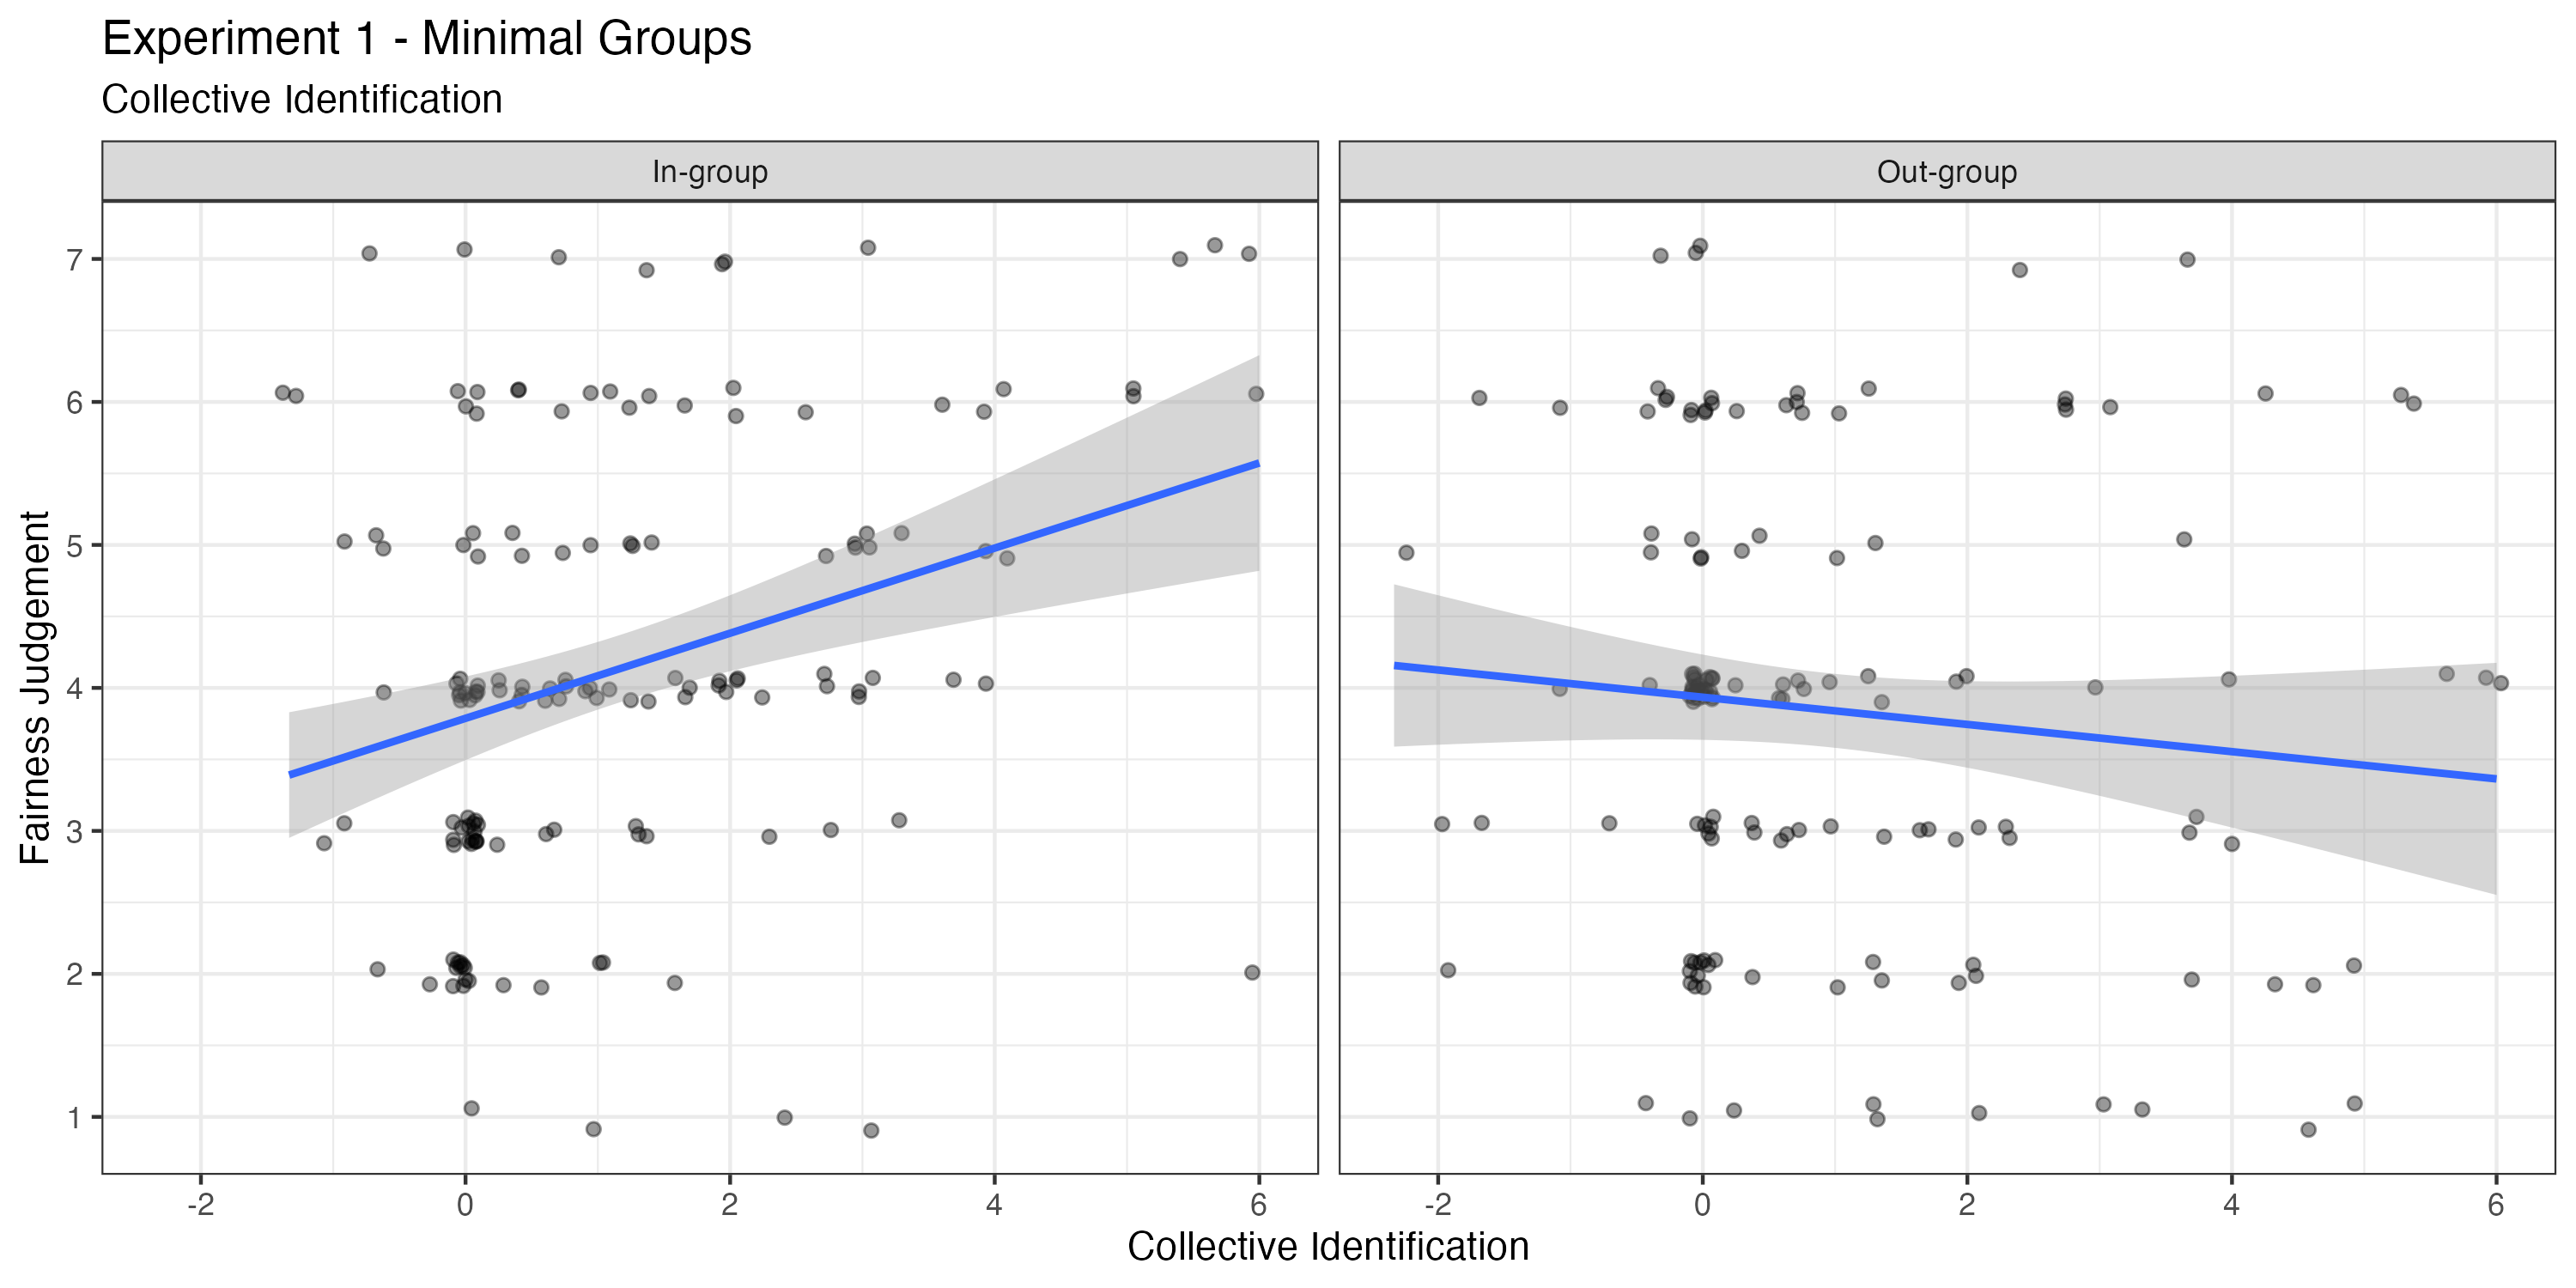
\includegraphics{Plots/Study1_CI_all.png}
	\caption{Scatterplot showing the relationship between Collective Identification with minimal group [Overestimator / Underestimator] fairness ratings of in-group members and out-group members immoral behavior. Collective identification is measured by calculating the difference score between 3-item in-group identification and 3 -item out-group identification. The fairness rating scale ran from 1 (very unfairly) to 7 (very fairly). The blue lines are regression coefficients, and the shaded region around the blue line represents the 95\% confidence interval. This graph shows all particiapnts, even those who reported higher identificaton with their out-group. Estimation results do not change when these participants are excluded. }
	\label{fig:CID_allS1}
\end{figure}


%%%%%%%%%%%%%%%%%%%%%%%%%%%%%%%%%%%%%%%%%%%%%%%%%%%%%%%%%%%%%%%%%%%%%%%%%%%%%%

\newpage
\subsection{Repeat Participants and Groups Excluded}
\label{appendix:repeat1}

Due to an error on Prolific, there were \emph{n} = 9 participants who participated in our study more than once. We exclude their repeated participations from analyses, but because this study involves both deception and participant interaction, it was possible that the repeat subjects could have revealed the purpose of the study to other participants during the chat phase. After examining the chat logs, we found repeat participants did not reveal the purpose of the study during the chats. Nonetheless, we ran a robustness check excluding all participants who chatted with a repeat participant \emph{n} = 33. Overall, we found that our results were robust even when excluding these participants.  

\begin{table}[ht]
\centering
\begin{tabular}{lrrrrr}
  \hline
 & Df & Sum Sq & Mean Sq & F value & Pr($>$F) \\ 
  \hline
Model & 3 & 23.66 & 7.89 & 3.82 & 0.0101 \\ 
  Contrast 1 - Self vs. Other & 1 & 3.09 & 3.09 & 1.50 & 0.2219 \\ 
  Contrast 2 - In-group vs. Out-group & 1 & 18.32 & 18.32 & 8.87 & 0.0030 \\ 
  Contrast 3 - Self/In-group vs. Other/Out-group & 1 & 2.25 & 2.25 & 1.09 & 0.2973 \\ 
  Risiduals & 499 & 1031.32 & 2.07 &  &  \\ 
   \hline
\end{tabular}
\caption{Results excluding those who had chatted with a repeat participant, \emph{n} = 503, altruists excluded. } 
\label{repeats_s1}
\end{table}

%%%%%%%%%%%%%%%%%%%%%%%%%%%%%%%%%%%%%%%%%%%%%%%%%%%%%%%%%%%%%%%%%%%%%%%%%%%%%%

\newpage
\subsection{Manipulation Check}
\label{appendix:manip1}

Because our study involved deception, it was critical that participants believe that they were (a) talking to real people during the chat phase. We pretested our paradigm in several pilot studies, and in our final sample for Study 1, we found that  75.34\% of participants believed they were talking to a real person during the chat phase of the experiment. As a robustness check, we found that our results did not change significantly, even when excluding those who failed our manipulation check. 

\vspace{0.6cm}

\begin{table}[ht]
\centering
\begin{tabular}{lrrrrr}
  \hline
 & Df & Sum Sq & Mean Sq & F value & Pr($>$F) \\ 
  \hline
Model & 3 & 16.73 & 5.58 & 2.19 & 0.0884 \\ 
  Contrast 1 - Self vs. Other & 1 & 7.67 & 7.67 & 3.02 & 0.0832 \\ 
  Contrast 2 - In-group vs. Out-group & 1 & 9.05 & 9.05 & 3.56 & 0.0599 \\ 
  Contrast 3 - Self/In-group vs. Other/Out-group & 1 & 0.00 & 0.00 & 0.00 & 0.9788 \\ 
  Risiduals & 402 & 1022.48 & 2.54 &  &  \\ 
   \hline
\end{tabular}
\caption{Only those who passed the manipulation check, \emph{n} = 334.} 
\label{manip}
\end{table}


%%%%%%%%%%%%%%%%%%%%%%%%%%%%%%%%%%%%%%%%%%%%%%%%%%%%%%%%%%%%%%%%%%%%%%%%%%%%%%

\clearpage
\section{Study 1 Exploratory Analyses}
\label{appendix:study1_robust}

%%%%%%%%%%%%%%%%%%%%%%%%%%%%%%%%%%%%%%%%%%%%%%%%%%%%%%%%%%%%%%%%%%%%%%%%%%%%%%

\subsection{Political Ideology and Extremity}
\label{appendix:ideo_extrem1}

\begin{figure}
	\centering
	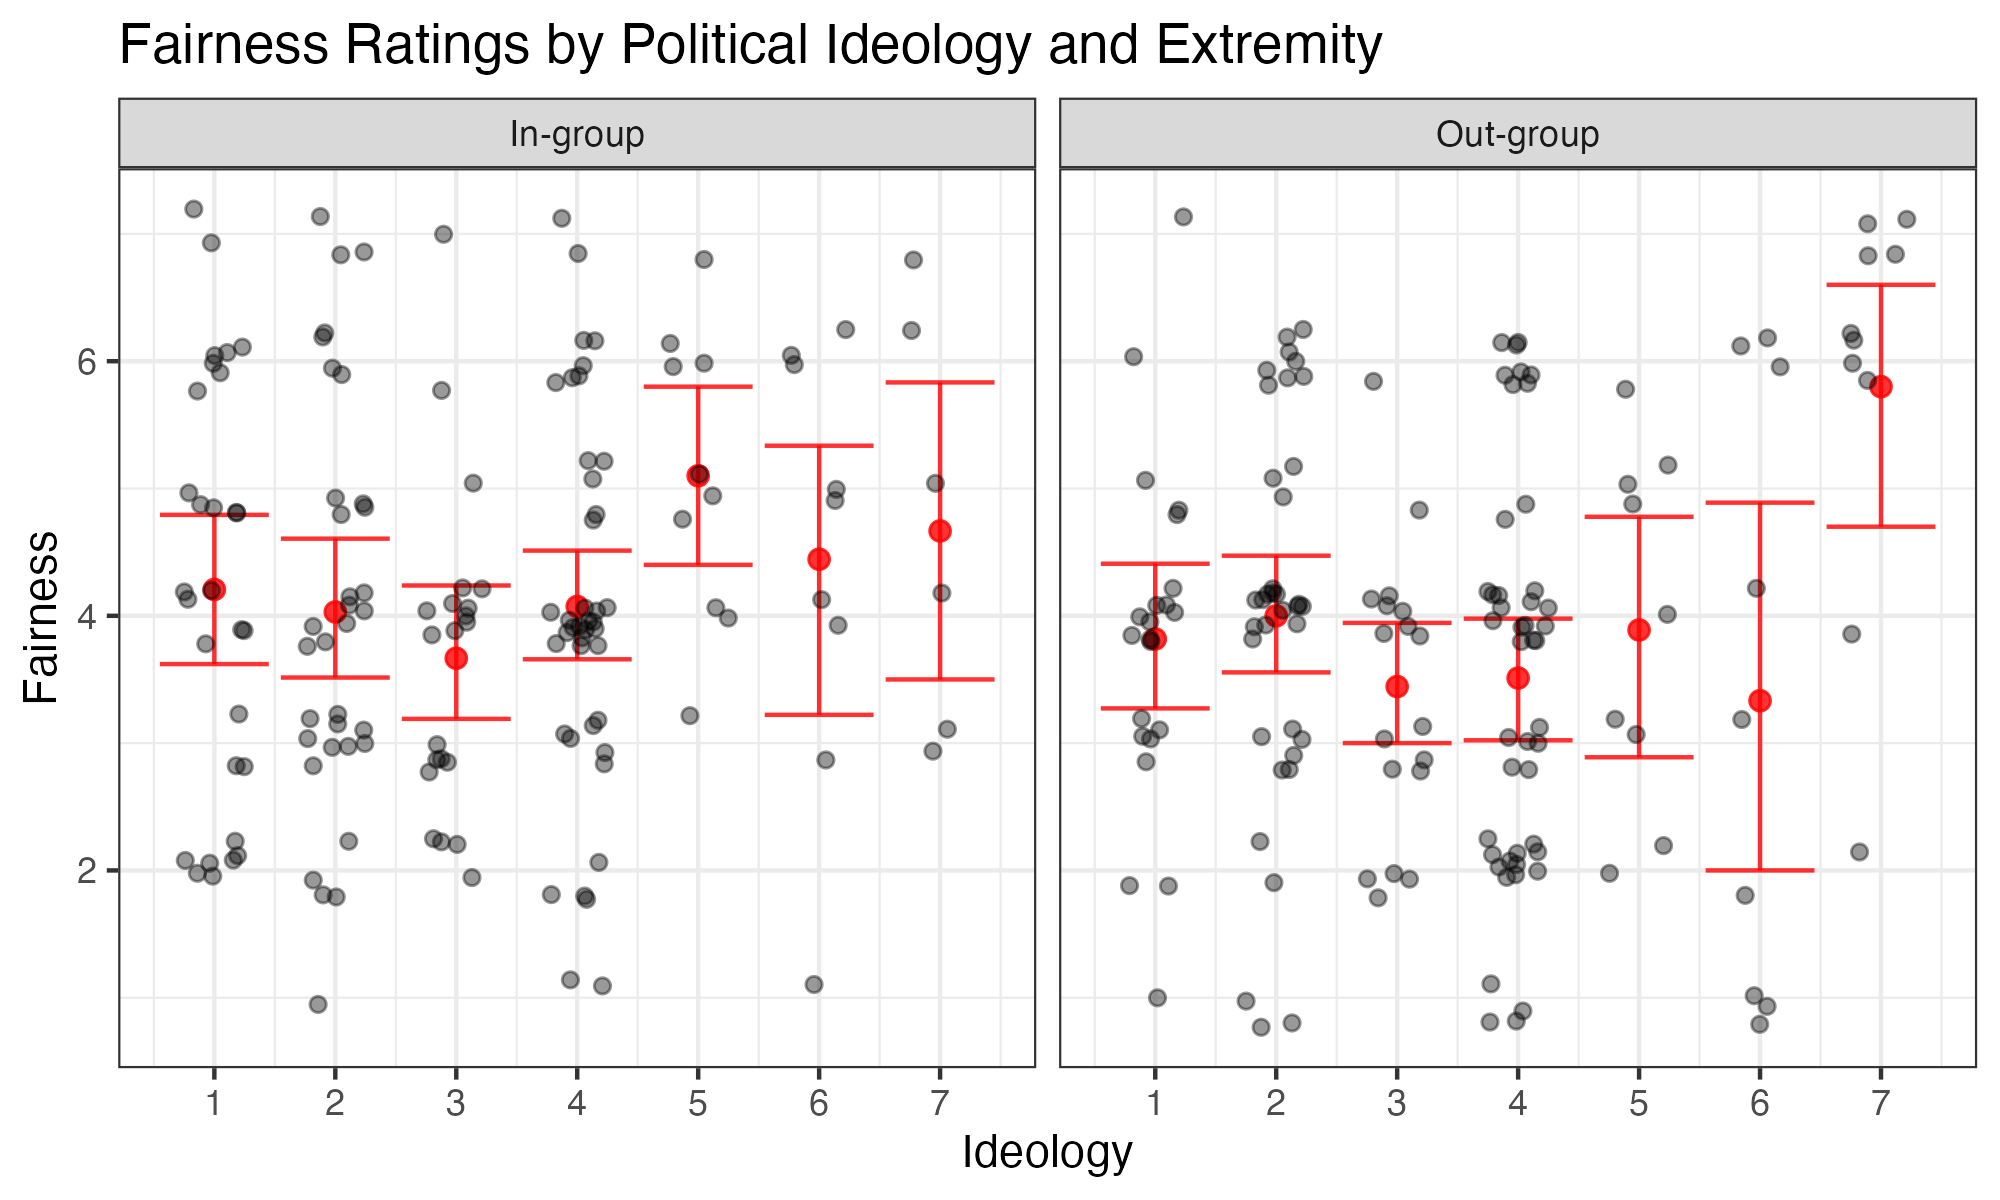
\includegraphics{Plots/Study1_ideology_extremity.png}
	\caption{Scatterplot showing fairness judgement ratings for in-group and out-group members by ideology. The fairness rating scale ran from 1 (very unfairly) to 7 (very fairly). Ideology was measured on a scale from 1 (very liberal) to 7 (very conservative). The red dots are means, and the red error bars represents the 95\% confidence interval.}
	\label{fig:CID_allS1}
\end{figure}


\begin{table}[ht]
\centering
\begin{tabular}{rrrrr}
  \hline
 & Estimate & Std. Error & t value & Pr($>$$|$t$|$) \\ 
  \hline
(Intercept) & 4.3594 & 0.4710 & 9.26 & 0.0000 \\ 
  Political Orientation & -0.2759 & 0.2953 & -0.93 & 0.3517 \\ 
  Political Orientation (Quadratic Term) & 0.0521 & 0.0405 & 1.29 & 0.2004 \\ 
   \hline
\end{tabular}
\caption{Effects of political ideology and extremity on on In-group Judgements } 
\label{ideo_ingroup1}
\end{table}


\clearpage


\begin{table}[ht]
\centering
\begin{tabular}{rrrrr}
  \hline
 & Estimate & Std. Error & t value & Pr($>$$|$t$|$) \\ 
  \hline
(Intercept) & 4.8436 & 0.5053 & 9.58 & 0.0000 \\ 
  Political Orientation & -0.8285 & 0.2979 & -2.78 & 0.0061 \\ 
  Political Orientation (Quadratic Term) & 0.1251 & 0.0385 & 3.25 & 0.0015 \\ 
   \hline
\end{tabular}
\caption{Effects of political ideology and extremity on on Out-group Judgements } 
\label{indeo_outgroup1}
\end{table}


%%%%%%%%%%%%%%%%%%%%%%%%%%%%%%%%%%%%%%%%%%%%%%%%%%%%%%%%%%%%%%%%%%%%%%%%%%%%%%

\clearpage
\subsection{High Identifiers Only}
\label{appendix:high_id1}

\begin{table}[ht]
\centering
\begin{tabular}{lrrrrr}
  \hline
 & Df & Sum Sq & Mean Sq & F value & Pr($>$F) \\ 
  \hline
Model & 3 & 37.83 & 12.61 & 4.55 & 0.0045 \\ 
  Contrast 1 - Self vs. Other & 1 & 9.66 & 9.66 & 3.49 & 0.0639 \\ 
  Contrast 2 - In-group vs. Out-group & 1 & 28.15 & 28.15 & 10.16 & 0.0018 \\ 
  Contrast 3 - Self/In-group vs. Other/Out-group & 1 & 0.03 & 0.03 & 0.01 & 0.9241 \\ 
  Risiduals & 138 & 382.26 & 2.77 &  &  \\ 
   \hline
\end{tabular}
\caption{Only particpants who scored greater than 2 on Collective Identification, \emph{n} = 142} 
\label{high_ID}
\end{table}

%%%%%%%%%%%%%%%%%%%%%%%%%%%%%%%%%%%%%%%%%%%%%%%%%%%%%%%%%%%%%%%%%%%%%%%%%%%%%%
%%%%%%% STUDY 2 STUDY 2 STUDY 2 %%%%%%%%%%%%%%%%%
%%%%%%%%%%%%%%%%%%%%%%%%%%%%%%%%%%%%%%%%%%%%%%%%%%%%%%%%%%%%%%%%%%%%%%%%%%%%%%

\newpage
\section{Study 2 Robustness Checks}
\label{appendix:robust2}

%%%%%%%%%%%%%%%%%%%%%%%%%%%%%%%%%%%%%%%%%%%%%%%%%%%%%%%%%%%%%%%%%%%%%%%%%%%%%%

\subsection{Intent to Treat Model}
\label{appendix:itt2}


\begin{table}[ht]
\centering
\begin{tabular}{lrrrrr}
  \hline
 & Df & Sum Sq & Mean Sq & F value & Pr($>$F) \\ 
  \hline
Model & 3 & 111.57 & 37.19 & 16.55 & 0.0000 \\ 
  Contrast 1 - Self vs. Other & 1 & 91.25 & 91.25 & 40.61 & 0.0000 \\ 
  Contrast 2 - In-group vs. Out-group & 1 & 16.77 & 16.77 & 7.46 & 0.0065 \\ 
  Contrast 3 - Self/In-group vs. Other/Out-group & 1 & 3.56 & 3.56 & 1.58 & 0.2086 \\ 
  Risiduals & 581 & 1305.57 & 2.25 &  &  \\ 
   \hline
\end{tabular}
\caption{Study 2: Intent-to-treat model, \emph{n} = 585. } 
\label{ITT2}
\end{table}



%%%%%%%%%%%%%%%%%%%%%%%%%%%%%%%%%%%%%%%%%%%%%%%%%%%%%%%%%%%%%%%%%%%%%%%%%%%%%%
\clearpage
\subsection{Differences in Overestimators and Underestimators}
\label{appendix:over_under2}

\begin{table}[ht]
\centering
\begin{tabular}{lrrrrr}
  \hline
 & Df & Sum Sq & Mean Sq & F value & Pr($>$F) \\ 
  \hline
Condition & 3 & 111.57 & 37.19 & 16.49 & 0.0000 \\ 
  Group (Overestimator or Underestimator) & 1 & 1.70 & 1.70 & 0.75 & 0.3854 \\ 
  Condition X Group & 3 & 2.17 & 0.72 & 0.32 & 0.8101 \\ 
  Risiduals & 577 & 1301.69 & 2.26 &  &  \\ 
   \hline
\end{tabular}
\caption{Differences between Overestimators and Underestimators in Study 2} 
\label{over_underS2}
\end{table}


Subsequent pairwise analyses demonstrated that fairness judgements of overestimators did not differ from underestimators in any condition -- the Self condition, \emph{t}(144.5) = 0.4257, \emph{p} = 0.671; the Other condition, \emph{t}(133.4) = -0.1535, \emph{p} = 0.878; the In-group condition, \emph{t}(144.8) = 1.306, \emph{p} = 0.194; or the Out-group condition, \emph{t}(132.8) = 0.1539, \emph{p} = 0.878. Equivalence testing was unable to conclude that these differences were not statistically different from zero -- Self condition,  \emph{t}(144.53) = -0.793, \emph{p} = 0.215; the Other condition, \emph{t}(131.4) = 1.029, \emph{p} = 0.153; the In-group condition, \emph{t}(144.8) = 0.0864, \emph{p} = 0.534; or the Out-group condition, \emph{t}(132.8) = -1.043, \emph{p} = 0.150


%%%%%%%%%%%%%%%%%%%%%%%%%%%%%%%%%%%%%%%%%%%%%%%%%%%%%%%%%%%%%%%%%%%%%%%%%%%%%%

\newpage
\subsection{Collective Identification with Out-group identifiers}
\label{appendix:mismatch}


Participants were assigned roles (either Democrats or Republicans) based on the ideology they reported on Prolific. We also asked participants to report their political orientation on a 7-point Likert scale (1 = Very Liberal, 7 = Very Conservative). We found that there were 5 participants who had reported that the were a Democrat on Prolific but responded that they were conservative in the survey, and 9 participants who reported that they were a Republican on Prolific, but responded that they were liberal in the survey. 

We also asked participants how much they identified with their political in-groups or out-groups in the survey, and found that there were 11 Democrats who reported identifying more with Republicans than Democrats, and 25 Republicans who reported identifying more with Democrats than Republicans. Results do not significantly change when these participants (\emph{n} = 46) are excluded.  Results from the contrast models are listed in \Cref{mismatch}. 


\vspace{0.6cm}

\begin{table}[ht]
\centering
\begin{tabular}{lrrrrr}
  \hline
 & Df & Sum Sq & Mean Sq & F value & Pr($>$F) \\ 
  \hline
Model & 3 & 29.16 & 9.72 & 4.75 & 0.0028 \\ 
  Contrast 1 - Self vs. Other & 1 & 2.38 & 2.38 & 1.16 & 0.2816 \\ 
  Contrast 2 - In-group vs. Out-group & 1 & 21.39 & 21.39 & 10.46 & 0.0013 \\ 
  Contrast 3 - Self/In-group vs. Other/Out-group & 1 & 5.39 & 5.39 & 2.64 & 0.1052 \\ 
  Risiduals & 482 & 985.87 & 2.05 &  &  \\ 
   \hline
\end{tabular}
\caption{Politically mismatched participants excluded, \emph{n} = 486.} 
\label{mismatch}
\end{table}

\clearpage

Results from the linear model examining the interaction effect between condition (In-group vs. Out-group) and Collective Identification was not significant $\beta$ = 0.086, \emph{t}(244) = 0.74, \emph{p} = 0.46. Graphs showing collective identification and fairness ratings with out-group identifiers included are in \cref{CID_allS2}

\vspace{0.5cm}

\begin{figure}
	\centering
	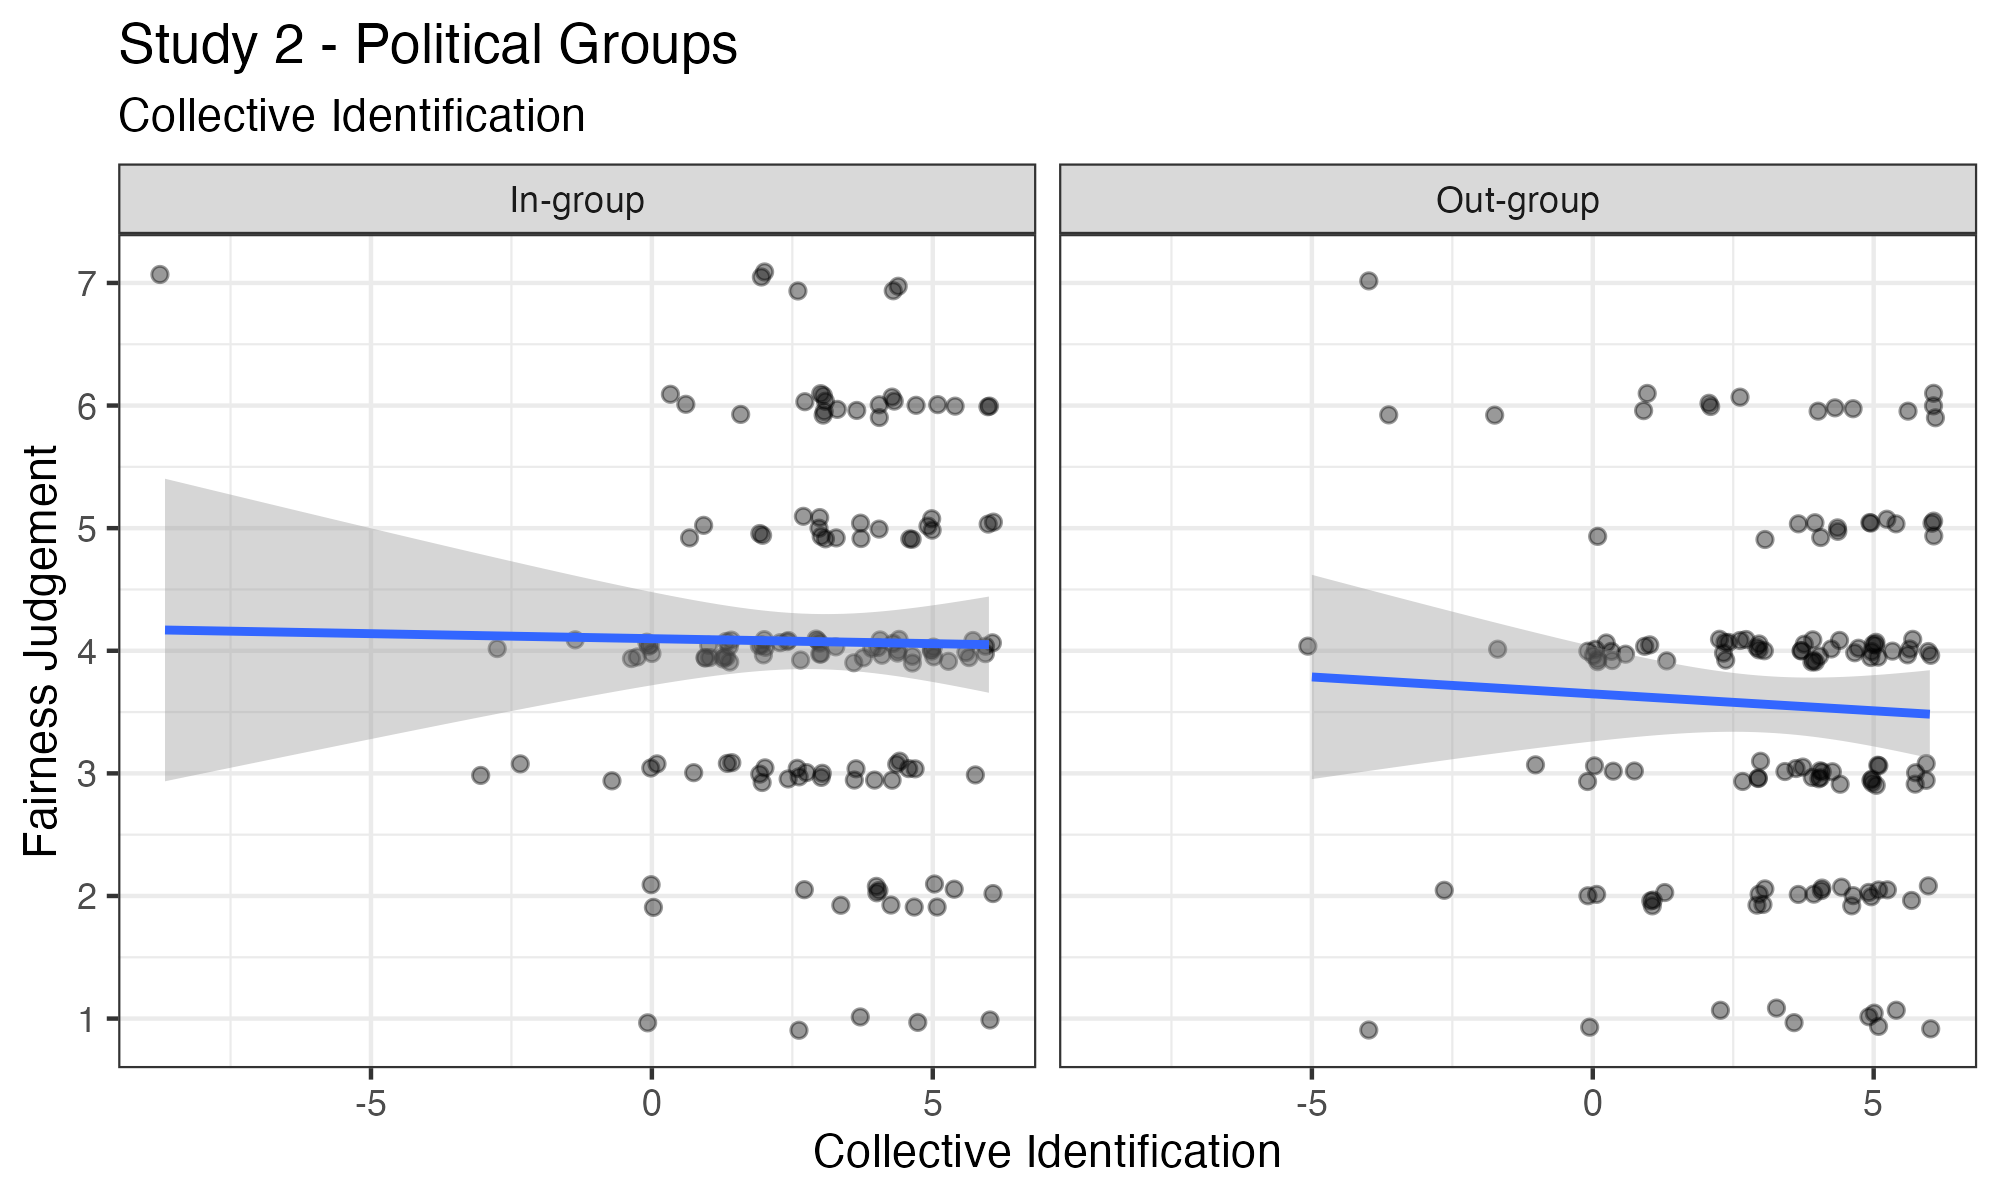
\includegraphics{Plots/Study2_CI_all.png}
	\caption{Scatterplot showing the relationship between Collective Identification with natural group [Democrat / Republican] fairness ratings of inigroup members and out-group members immoral behavior. Collective identification is measured by calculating the difference score between 3-item in-group identification and 3 -item out-group identification.The fairness rating scale ran from 1 (very unfairly) to 7 (very fairly). The blue lines are regression coefficients, and the shaded region around the blue line represents the 95\% confidence interval. This graph shows all participants, even those who reported higher identification with their out-group. Estimation results do not change when these participants are excluded. }
	\label{fig:CID_allS2}
\end{figure}





%%%%%%%%%%%%%%%%%%%%%%%%%%%%%%%%%%%%%%%%%%%%%%%%%%%%%%%%%%%%%%%%%%%%%%%%%%%%%%

\newpage
\subsection{Repeat Participants and Groups Excluded}
\label{appendix:exclude}

Due to an error on Prolific, there were \emph{n} = 13 participants who participated in our study more than once. We exclude their repeated participations from analyses, but because this study involves both deception and participant interaction, it was possible that the repeat subjects could have revealed the purpose of the study to other participants during the chat phase. After examining the chat logs, we found repeat participants did not reveal the purpose of the study during the chats. Nonetheless, we ran a robustness check excluding all participants who chatted with a repeat participant \emph{n} = 45. Overall, we found that our results were robust even when excluding these participants.  

\vspace{0.6cm}

\begin{table}[ht]
\centering
\begin{tabular}{lrrrrr}
  \hline
 & Df & Sum Sq & Mean Sq & F value & Pr($>$F) \\ 
  \hline
Model & 3 & 23.66 & 7.89 & 3.82 & 0.0101 \\ 
  Contrast 1 - Self vs. Other & 1 & 3.09 & 3.09 & 1.50 & 0.2219 \\ 
  Contrast 2 - In-group vs. Out-group & 1 & 18.32 & 18.32 & 8.87 & 0.0030 \\ 
  Contrast 3 - Self/In-group vs. Other/Out-group & 1 & 2.25 & 2.25 & 1.09 & 0.2973 \\ 
  Risiduals & 499 & 1031.32 & 2.07 &  &  \\ 
   \hline
\end{tabular}
\caption{Results excluding those who had chatted with a repeat participant, \emph{n} = 503, altruists excluded.} 
\label{repeats}
\end{table}

%%%%%%%%%%%%%%%%%%%%%%%%%%%%%%%%%%%%%%%%%%%%%%%%%%%%%%%%%%%%%%%%%%%%%%%%%%%%%%

\newpage
\subsection{Manipulation Check}
\label{appendix:manip2}

Because our study involved deception, it was critical that participants believe that they were (a) talking to real people during the chat phase and (b) that they were seeing a real person's choice behavior. We pretested our paradigm in several pilot studies, and in our final sample for Study 2, we found that  73.97\% of participants believed they were talking to a real person during the chat phase of the experiment, and 74.48 \% of participants in Conditions 2, 3, and 4 believed that another participant really was assigning tasks. As a robustness check, we found that our results were robust even when excluding those who failed both manipulation checks. 

\vspace{0.6cm}

\begin{table}[ht]
\centering
\begin{tabular}{lrrrrr}
  \hline
 & Df & Sum Sq & Mean Sq & F value & Pr($>$F) \\ 
  \hline
Model & 3 & 15.83 & 5.28 & 2.54 & 0.0568 \\ 
  Contrast 1 - Self vs. Other & 1 & 0.23 & 0.23 & 0.11 & 0.7419 \\ 
  Contrast 2 - In-group vs. Out-group & 1 & 12.54 & 12.54 & 6.03 & 0.0146 \\ 
  Contrast 3 - Self/In-group vs. Other/Out-group & 1 & 3.06 & 3.06 & 1.47 & 0.2263 \\ 
  Risiduals & 305 & 634.06 & 2.08 &  &  \\ 
   \hline
\end{tabular}
\caption{Only those who passed the manipulation check, \emph{n} = 309.} 
\label{manip2}
\end{table}

%%%%%%%%%%%%%%%%%%%%%%%%%%%%%%%%%%%%%%%%%%%%%%%%%%%%%%%%%%%%%%%%%%%%%%%%%%%%%%
%%%%%%%%%%%%%%%%%%%%%%%%%%%%%%%%%%%%%%%%%%%%%%%%%%%%%%%%%%%%%%%%%%%%%%%%%%%%%%


\clearpage
\section{Study 2 Exploratory Analyses}
\label{appendix:explore2}


%%%%%%%%%%%%%%%%%%%%%%%%%%%%%%%%%%%%%%%%%%%%%%%%%%%%%%%%%%%%%%%%%%%%%%%%%%%%%%

\subsection{Political Ideology and Extremity}
\label{appendix:ideo_extrem2}


\begin{figure}
	\centering
	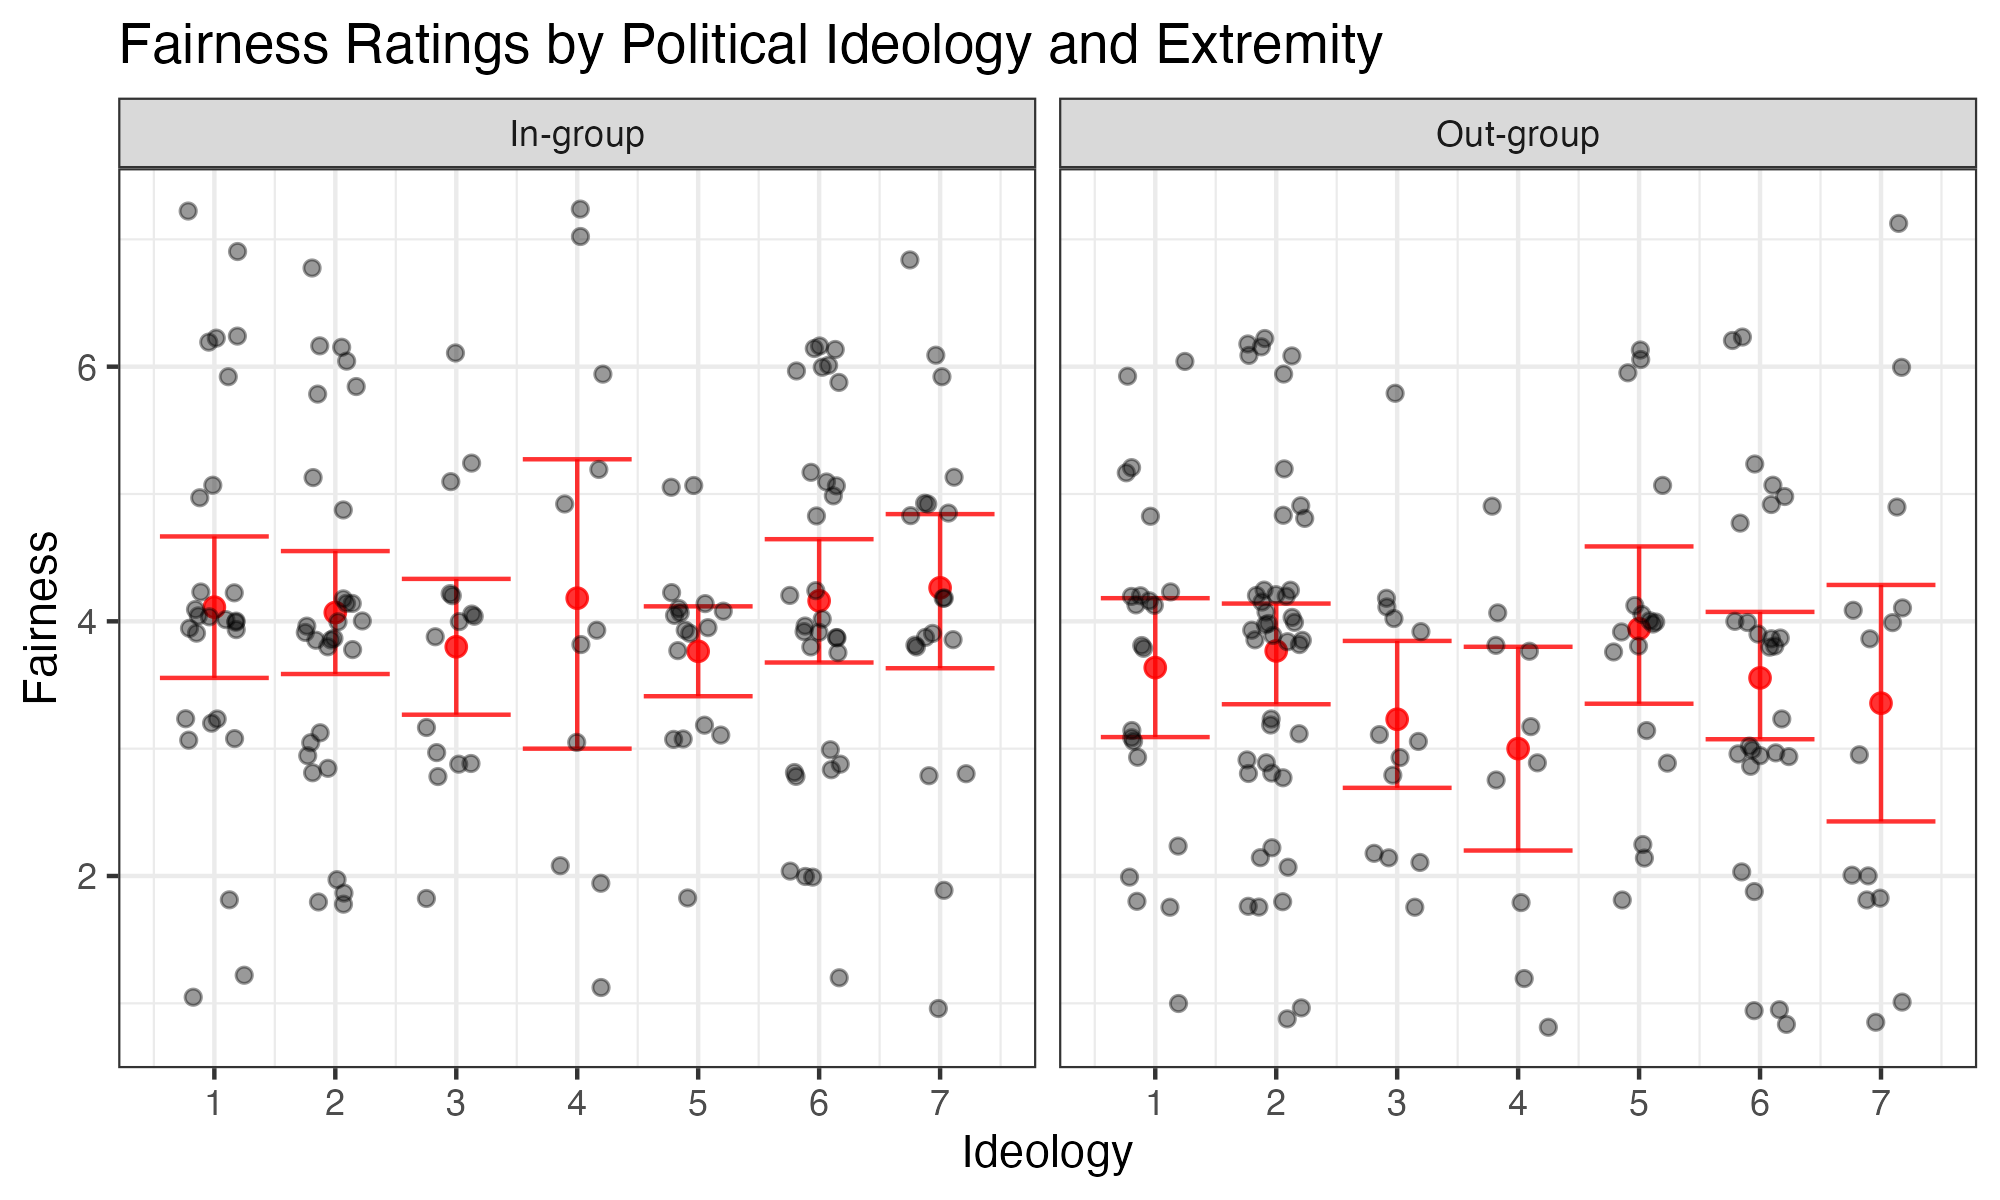
\includegraphics{Plots/Study2_ideology_extremity.png}
	\caption{Scatterplot showing fairness judgement ratings for in-group and out-group members by ideology. The fairness rating scale ran from 1 (very unfairly) to 7 (very fairly). Ideology was measured on a scale from 1 (very liberal) to 7 (very conservative). The red dots are means, and the red error bars represents the 95\% confidence interval.}
	\label{fig:CID_allS1}
\end{figure}


\begin{table}[ht]
\centering
\begin{tabular}{rrrrr}
  \hline
 & Estimate & Std. Error & t value & Pr($>$$|$t$|$) \\ 
  \hline
(Intercept) & 4.3397 & 0.4423 & 9.81 & 0.0000 \\ 
  Political Orientation & -0.2314 & 0.2791 & -0.83 & 0.4085 \\ 
  Political Orientation (Quadratic Term) & 0.0318 & 0.0350 & 0.91 & 0.3648 \\ 
   \hline
\end{tabular}
\caption{Effects of political ideology and extremity on on In-group Judgements. } 
\label{ideo_ingroup2}
\end{table}

\clearpage

\begin{table}[ht]
\centering
\begin{tabular}{rrrrr}
  \hline
 & Estimate & Std. Error & t value & Pr($>$$|$t$|$) \\ 
  \hline
(Intercept) & 3.7458 & 0.4837 & 7.74 & 0.0000 \\ 
  Political Orientation & -0.0614 & 0.3065 & -0.20 & 0.8414 \\ 
  Political Orientation (Quadratic Term) & 0.0038 & 0.0386 & 0.10 & 0.9209 \\ 
   \hline
\end{tabular}
\caption{Effects of political ideology and extremity on on Out-group Judgements .} 
\label{ideo_outgroup2}
\end{table}




%%%%%%%%%%%%%%%%%%%%%%%%%%%%%%%%%%%%%%%%%%%%%%%%%%%%%%%%%%%%%%%%%%%%%%%%%%%%%%

\clearpage
\subsection{Partisan Differences}
\label{appendix:p_dif2}

We did not preregister any partisan differences, but we also wanted to include an exploratory analysis comparing Democrats and Republicans.  We find evidence of out-group derogation, but not moral hypocrisy in Democrats, whereas we find evidence of both out-group derogation and moral hypocrisy in Republicans. 

\vspace{0.6cm}

\begin{table}[ht]
\centering
\begin{tabular}{lrrrrr}
  \hline
 & Df & Sum Sq & Mean Sq & F value & Pr($>$F) \\ 
  \hline
Model & 3 & 11.08 & 3.69 & 1.96 & 0.1198 \\ 
  Contrast 1 - Self vs. Other & 1 & 3.14 & 3.14 & 1.67 & 0.1976 \\ 
  Contrast 2 - In-group vs. Out-group & 1 & 7.88 & 7.88 & 4.19 & 0.0417 \\ 
  Contrast 3 - Self/In-group vs. Other/Out-group & 1 & 0.07 & 0.07 & 0.04 & 0.8505 \\ 
  Risiduals & 264 & 496.63 & 1.88 &  &  \\ 
   \hline
\end{tabular}
\caption{Democrats only, \emph{n} = 268.} 
\label{dems2}
\end{table}

\vspace{0.6cm}

\begin{table}[ht]
\centering
\begin{tabular}{lrrrrr}
  \hline
 & Df & Sum Sq & Mean Sq & F value & Pr($>$F) \\ 
  \hline
Model & 3 & 39.75 & 13.25 & 6.12 & 0.0005 \\ 
  Contrast 1 - Self vs. Other & 1 & 20.35 & 20.35 & 9.41 & 0.0024 \\ 
  Contrast 2 - In-group vs. Out-group & 1 & 10.76 & 10.76 & 4.97 & 0.0266 \\ 
  Contrast 3 - Self/In-group vs. Other/Out-group & 1 & 8.64 & 8.64 & 3.99 & 0.0467 \\ 
  Risiduals & 260 & 562.40 & 2.16 &  &  \\ 
   \hline
\end{tabular}
\caption{Republicans only, \emph{n} = 264. } 
\label{reps2}
\end{table}



\end{document}